%
% Portuguese-BR vertion
% 
\documentclass{report}

\usepackage{ipprocess}
% Use longtable if you want big tables to split over multiple pages.
\usepackage{longtable}
\usepackage[utf8]{inputenc} 
\usepackage[brazil]{babel} % Uncomment for portuguese
\usepackage{pdflscape} % set ladscape/portrait pdf pages
\usepackage{tikz}
\usepackage{tikz-uml}

\sloppy

\graphicspath{{./pictures/}} % Pictures dir
\makeindex
\begin{document}


%%%%%%%%%%%%%%%%%%%%%%%%%%%%%%%%%%%%%%%%%%%%%%%%%%
%% Building front cover
%%%%%%%%%%%%%%%%%%%%%%%%%%%%%%%%%%%%%%%%%%%%%%%%%%
\DocumentTitle{Documento de Arquitetura}
\Project{Unidade de Operações Aritméticas}
\Organization{Universidade Estadual de Feira de Santana}
\Version{Compilação 1.0}
% Make front cover
\capa
%

%%%%%%%%%%%%%%%%%%%%%%%%%%%%%%%%%%%%%%%%%%%%%%%%%%
%% Revision History
%%%%%%%%%%%%%%%%%%%%%%%%%%%%%%%%%%%%%%%%%%%%%%%%%%
\chapter*{Histórico de Revisões}
  \vspace*{1cm}
  \begin{table}[ht]
    \centering
    \begin{tabular}[pos]{|m{2cm} | m{8cm} | m{4cm}|} 
      \hline
      \cellcolor[gray]{0.9}
      \textbf{Date} & \cellcolor[gray]{0.9}\textbf{Descrição} & \cellcolor[gray]{0.9}\textbf{Autor(s)}\\
      \hline
      25/06/2014 &  Concepção do documento & joaocarlos \\ \hline
      15/10/2014 &  Adição da subseção de acesso à memória & Weverson Gomes \\ \hline
      16/10/2014 &  Adição da subseção de acesso à memória & Weverson Gomes \\ \hline
    \end{tabular}
  \end{table}

% TOC instantiation
\tableofcontents

%%%%%%%%%%%%%%%%%%%%%%%%%%%%%%%%%%%%%%%%%%%%%%%%%%
%% Document main content
%%%%%%%%%%%%%%%%%%%%%%%%%%%%%%%%%%%%%%%%%%%%%%%%%%
\chapter{Introdução}
  
	\section{Introdução}

 A \textbf{Fazemos Qualquer Negócio Inc.} foi contratada para o desenvolvimento do \textit{IP-Core} \textbf{MUSA}, que é um micro processador de
 propósito geral que será utilizado em escolas de países africanos com o intuito de impulsionar o desenvolvimento deste continente. As seções
 subsequentes apresentam os requisitos funcionais e não funcionais como parte da fase de \textbf{Concepção} do IP-process.
 Os requisitos listados foram definidos a partir das necessidades do cliente para produção do \textit{MUSA}.

\chapter{Visão Geral da Arquitetura}

	\section{Restrições}
	\begin{itemize}
	\item \textbf{Restrições --} %fazer junto com os desenvolvedores
	\end{itemize}
	
	\section{Codificação das instruções}
	Instrução é uma palavra da linguagem de máquina, sua codificação é de fundamental importância para o processamento das operações.	Todas as instruções contém 32 bits. Exitem 4 formatos de instruções: R (R-type), I (I-type), Load/Store e Jump. Os OPCODES são os códigos de operação da instrução, neste documento ele é representação em números hexadecimais.\\
	
  \FloatBarrier
    \begin{center}
\begin{longtable}[pos]{| c | c | c | m{7cm} |} \hline    
          \multicolumn{1}{|c|}{\cellcolor[gray]{0.9}\textbf{Formato da instrução}} & 
          \multicolumn{1}{c|}{\cellcolor[gray]{0.9}\textbf{Instrução}} & 
          \multicolumn{1}{c|}{\cellcolor[gray]{0.9}\textbf{Descrição}} \\ \hline
          \endfirsthead
          \hline
          \multicolumn{3}{|l|}
          {{\bfseries continuação da página anterior}} \\
          \hline
          \multicolumn{1}{|c|}{\cellcolor[gray]{0.9}\textbf{Formato da Instrução}} & 
          \multicolumn{1}{c|}{\cellcolor[gray]{0.9}\textbf{Instrução}} & 
          \multicolumn{1}{c|}{\cellcolor[gray]{0.9}\textbf{Descrição}} \\ \hline
          \endhead

          \multicolumn{3}{|r|}{{continua na próxima página}} \\ \hline
          \endfoot

          \hline
          \endlastfoot 
           
			\multirow{8}{*}{R-type} & ADD & Soma dois valores \\ \cline{2-3}	
	& SUB & Subtrai dois valores \\ \cline{2-3}	
	& MUL & Multiplica dois valores \\ \cline{2-3}	
	& DIV & Divide dois valores \\ \cline{2-3}
	& AND & AND lógico \\ \cline{2-3}
	& OR & OR lógico  \\ \cline{2-3}
	& CMP & Compara dois valores \\ \cline{2-3}
	& NOT & NOT lógico \\ \hline 
	\multirow{4}{*}{I-type} & ADDI & Soma dois valores,um destes imediato. \\ \cline{2-3}
	& SUBI & Subtrai dois valores, um destes imediato. \\ \cline{2-3}
	& ANDI & AND lógico de dois valores, um destes imediato. \\ \cline{2-3}
	& ORI & OR lógico de dois valores, um destes imediato. \\ \cline{2-3}
	& LW & Leitura de um dado da memória de dados \\ \cline{2-3}
	& SW & Armazena um dado na memória de dados \\ \hline
	\multirow{6}{*}{Jump} & JP & Desvia para um destino \\ \cline{2-3}
	& JPC & Desvia para um destino relativo ao PC \\ \cline{2-3}
	& BRFL & Desvia para um destino se RF==CST \\ \cline{2-3}
	& CALL & Chamada de subrotina \\ \cline{2-3}
	& RET & Retorno de Subrotina \\ \cline{2-3}
	& HALT & Parada do sistema \\ \cline{2-3}
	& NOPE & Refresh no módulo \\ \hline
\end{longtable}
\end{center}


	O formato R está relacionado as instruções lógicas e aritméticas.
	\begin{figure}[H]
    	\centering
    	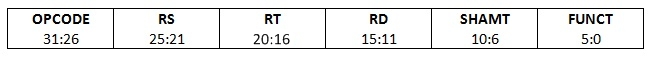
\includegraphics{r-format}
    	\caption{Formato R}
		\label{r_format}
	\end{figure}
	Seus respectivos campos são:
	\begin{itemize}
	\item \textbf{OPCODE} - Código da operação básica da instrução.
	\item \textbf{RS} - Registrador do primeiro operando de origem.
	\item \textbf{RT} - Registrador do segundo operando de origem.
	\item \textbf{RD} - Registrador destino.
	\item \textbf{SHAMT} - \textit{Shift amount}; Quantidade de deslocamento.
	\item \textbf{FUNCT} - Função; Esse campo seleciona a variante específica da operação no campo opcode, e as vezes, é chamado de código de função.
\end{itemize}	

\begin{table}[H]
\centering
	\begin{tabular}{|c|c|c|}
  	\hline 
  	\cellcolor[gray]{0.9}\textbf{OPCODE} & \cellcolor[gray]{0.9}\textbf{INSTRUCTION} & \cellcolor[gray]{0.9}\textbf{FUNCTION} \\ 
  	\hline 
  	0x00 & ADD & 0x20 \\ 
  	\hline 
  	0x00 & SUB & 0x22 \\ 
  	\hline 
  	0x00 & MUL & 0x18 \\ 
  	\hline 
  	0x00 & DIV & 0x1A \\ 
  	\hline 
  	0x00 & AND & 0x24 \\ 
  	\hline 
  	0x00 & OR & 0x25 \\ 
  	\hline 
  	0x00 & CMP & 0x1C \\ 
  	\hline 
  	0x00 & NOT & 0x1D \\ 
  	\hline 
  	\end{tabular} 
  	\caption{Definição dos OPCODES do formato R}
  \end{table} 
  	 	
  	
	 Um segundo tipo de formato de instrução é chamado de formato I, utilizado pelas instruções imediatas e de transferência de dados.
	\begin{figure}[H]
    	\centering
    	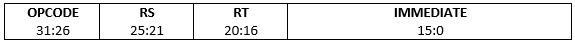
\includegraphics{i-format}
    	\caption{Formato I}
		\label{i_format}
  	\end{figure}
Seus respectivos campos são:
	\begin{itemize}
	\item \textbf{OPCODE} - Código da operação básica da instrução.
	\item \textbf{RS} - Registrador do operando de origem.
	\item \textbf{RT} - Registrador destino.
	\item \textbf{ADDRESS OR IMMEDIATE} - Endereço de memória ou constante numérica.
\end{itemize}	  	

\begin{table}[H]
\centering	
\begin{tabular}{|c|c|}
	\hline 
  	\cellcolor[gray]{0.9}\textbf{OPCODE} & \cellcolor[gray]{0.9}\textbf{INSTRUCTION} \\ 
	\hline 
	0x08 & ADDI \\ %
	\hline 
	0x10 & SUBI \\ %
	\hline 
	0x0c & ANDI \\ %
	\hline 
	0x13 & ORI \\ %
	\hline 
	0x23 & LW \\ %
	\hline 
	0x2b & SW \\ %	
%	0x2a
%0x04
%0x04
	\hline 
	\end{tabular} 
	  	\caption{Definição dos OPCODES do formato I}	
\end{table}	
	
 O formato Jump servem para as instruções de desvio incondicional.  	
   	\begin{figure}[H]
    	\centering
    	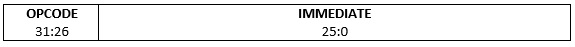
\includegraphics{jump}
    	\caption{Formato Jump}
		\label{jump}
  	\end{figure}
Seus respectivos campos são:
	\begin{itemize}
	\item \textbf{OPCODE} - Código da operação básica da instrução.
	\item \textbf{ADDRESS} - Endereço de memória ou constante numérica.
\end{itemize}
 
\begin{table}[H]
\centering 	
  	\begin{tabular}{|c|c|}
  	\hline 
  	\cellcolor[gray]{0.9}\textbf{OPCODE} & \cellcolor[gray]{0.9}\textbf{INSTRUCTION} \\ 
  	\hline 
  	- & JP \\ 
  	\hline 
  	- & JPC \\ 
  	\hline 
  	0x09 & BRFL \\ 
  	\hline 
  	- & CALL \\ 
  	\hline 
  	- & RET \\ 
  	\hline 
  	- & HALT \\ 
  	\hline 
  	- & NOPE \\ 
  	\hline 
  	\end{tabular} 
  	  	\caption{Definição dos OPCODES do formato Jump}
\end{table}
	
	\section{Descrição dos Componentes}
  A unidade de processamento a ser desenvolvida é composta a partir dos seguintes componentes:

  \begin{itemize}
    \item \textbf{Instruction Fetch --} Módulo responsavel pela busca da instrução na memória de instrução.
    \item \textbf{Instruction Decode e Register Read --} Módulo responsável pela decodificação das instruções e leitura do banco de registradores.
    \item \textbf{Execute Operation or Calculate Address --} Módulo responsável pela execução as operações de caractér lógico/aritmético ou cálculos endereços.
     \item \textbf{Memory Access e Write Back --} Módulo responsável pelo acesso a memória de dados e escrita no banco de registradores.
  \end{itemize}

  \section{Diagrama de Classe (Interface)}
  \begin{figure}[H]
    \centering
        \begin{tikzpicture} 
      \umlclass[type=interface]{IP\_Interface}
      { % atributos
        + clock : input bit \\
        + reset : input bit \\
        + rx : input bit \\
        % + tx : output bit \\
        + result\_data : output bit[8] \\
        + overflow : output bit
      }{}
    \end{tikzpicture}
  \end{figure}

  \section{Definições de Entrada e Saída}
  \FloatBarrier
    \begin{center}
      \begin{longtable}[pos]{| l | c | c | m{7cm} |} \hline         
        \multicolumn{1}{|c|}{\cellcolor[gray]{0.9}\textbf{Nome}} & 
        \multicolumn{1}{c|}{\cellcolor[gray]{0.9}\textbf{Tamanho}} & 
        \multicolumn{1}{c|}{\cellcolor[gray]{0.9}\textbf{Direção}} &
        \multicolumn{1}{c|}{\cellcolor[gray]{0.9}\textbf{Descrição}} \\ \hline
        \endfirsthead
        \hline
        \multicolumn{4}{|l|}%
        {{\bfseries continuação da página anterior}} \\
        \hline
        \multicolumn{1}{|c|}{\cellcolor[gray]{0.9}\textbf{Nome}} & 
        \multicolumn{1}{c|}{\cellcolor[gray]{0.9}\textbf{Tamanho}} & 
        \multicolumn{1}{c|}{\cellcolor[gray]{0.9}\textbf{Direção}} &
        \multicolumn{1}{c|}{\cellcolor[gray]{0.9}\textbf{Descrição}} \\ \hline
        \endhead

        \multicolumn{4}{|r|}{{continua na próxima página}} \\ \hline
        \endfoot

        \hline
        \endlastfoot

        clock\_in                & 1   & entrada   & Clock principal do sistema.    \\ \hline
        reset\_in                & 1   & entrada   & Sinal de reset geral do sistema.    \\ \hline
        rx\_in                   & 1   & entrada   & Dado serial da RS232. \\ \hline
        % tx\_out                  & 1   & saída     & Dado serial RS232 a ser transmitido. \\ \hline
        result\_data\_out        & 8   & saída     & Representação do resultado da operação. \\ \hline
        overflow\_out            & 1   & saída     & Sinal indicador de overflow aritmético. \\
      \end{longtable}
    \end{center} 
  \section{Datapath Interno}
    \begin{figure}[H]
      \centering
      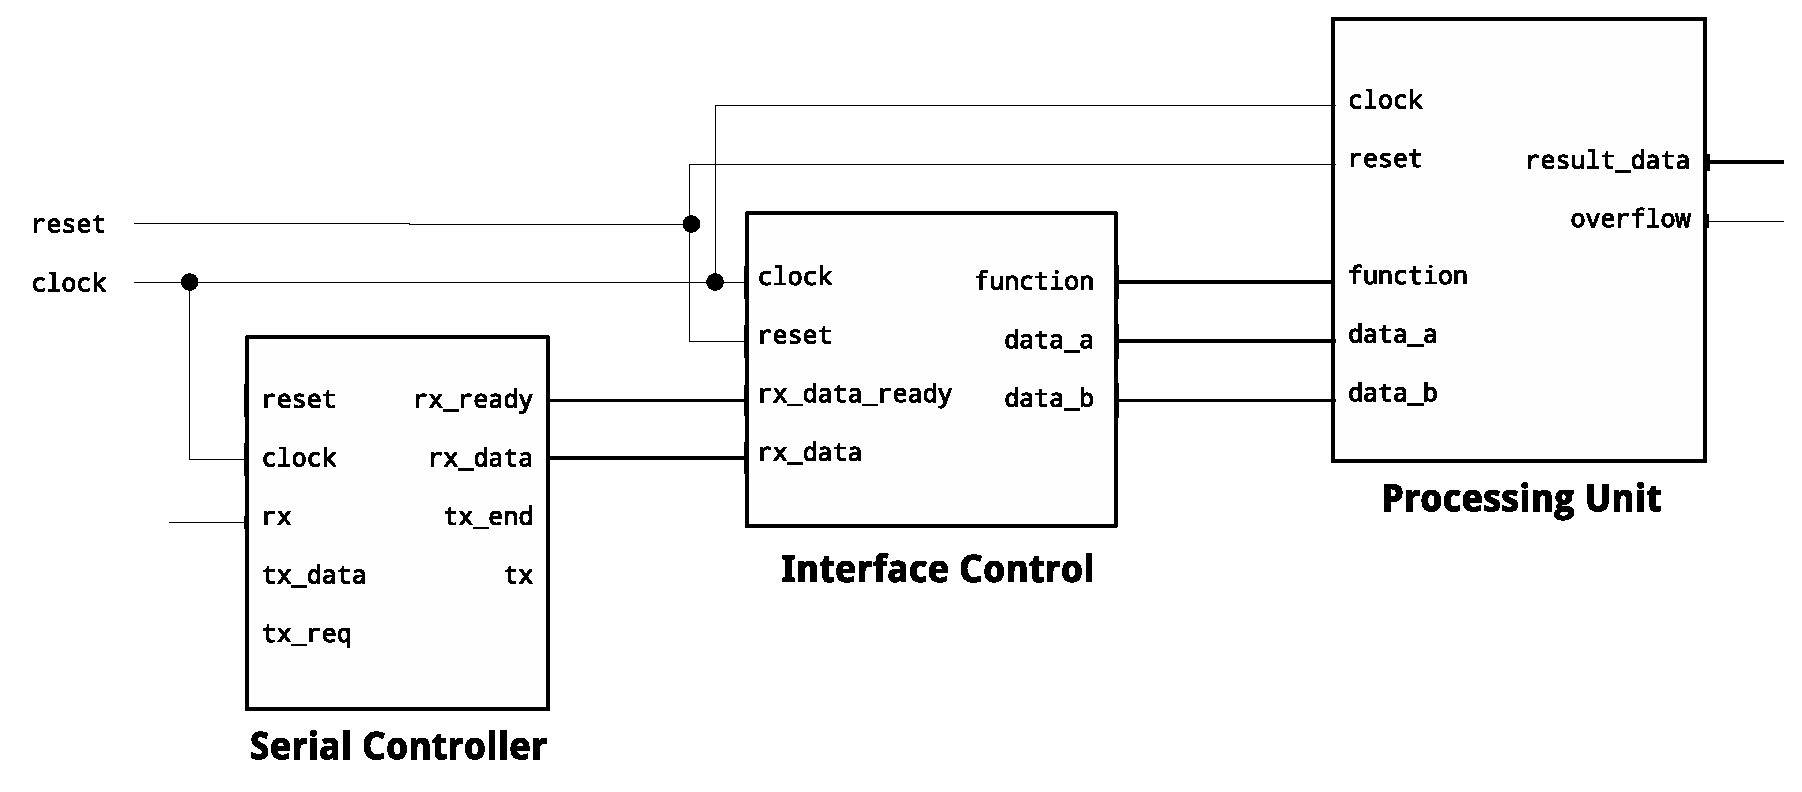
\includegraphics[width=\linewidth]{datapath/ip_datapath.eps}
    \end{figure}

% inicio das descrições de arquitetura para cada componente do sistema
\chapter{Descrição da Arquitetura}

	  \section{Unidade de Processamento}

    \subsection{Diagrama de Classe}
      \begin{figure}[H]
      \centering
            \begin{tikzpicture} 
        \umlclass[type=control]{Processing\_Unit}
        { % atributos
          + clock : input bit \\
          + reset : input bit \\
          + data\_a : input bit[8] \\
          + data\_b : input bit[8] \\
          + operation : input bit[TBD] \\          
          + result\_data : output bit[8] \\
          + overflow : output bit \\
          - enable\_result\_reg : reg bit \\
          - reult\_reg : reg bit[8]
        }{ % procedures
          - \underline{<<comb>> process\_operation()} \\
          - <<comb>> setup\_flag() \\
          - <<sequ>> result\_reg\_handler()
        }
      \end{tikzpicture}
    \end{figure}

    \subsection{Definições de Entrada e Saída}
      \FloatBarrier
      \begin{center}
        \begin{longtable}[pos]{| l | c | c | m{7cm} |} \hline         
          \multicolumn{1}{|c|}{\cellcolor[gray]{0.9}\textbf{Nome}} & 
          \multicolumn{1}{c|}{\cellcolor[gray]{0.9}\textbf{Tamanho}} & 
          \multicolumn{1}{c|}{\cellcolor[gray]{0.9}\textbf{Direção}} &
          \multicolumn{1}{c|}{\cellcolor[gray]{0.9}\textbf{Descrição}} \\ \hline
          \endfirsthead
          \hline
          \multicolumn{4}{|l|}%
          {{\bfseries continuação da página anterior}} \\
          \hline
          \multicolumn{1}{|c|}{\cellcolor[gray]{0.9}\textbf{Nome}} & 
          \multicolumn{1}{c|}{\cellcolor[gray]{0.9}\textbf{Tamanho}} & 
          \multicolumn{1}{c|}{\cellcolor[gray]{0.9}\textbf{Direção}} &
          \multicolumn{1}{c|}{\cellcolor[gray]{0.9}\textbf{Descrição}} \\ \hline
          \endhead

          \multicolumn{4}{|r|}{{continua na próxima página}} \\ \hline
          \endfoot

          \hline
          \endlastfoot

          clock\_in                & 1   & entrada   & Clock principal do sistema.    \\ \hline
          reset\_in                & 1   & entrada   & Sinal de reset geral do sistema.    \\ \hline
          data\_a\_in              & 8   & entrada   & Dado do primeiro operando.    \\ \hline
          data\_b\_in              & 8   & entrada   & Dado do segundo operando.    \\ \hline
          operation\_in            & TBD   & entrada   & Código da operação.    \\ \hline
          result\_data\_out        & 8   & saída     & Representação do resultado da operação. \\ \hline
          overflow\_out            & 1   & saída     & Sinal indicador de overflow aritmético. \\
        \end{longtable}
      \end{center} 

    \subsection{Datapath Interno}
      \begin{figure}[H]
        \centering
        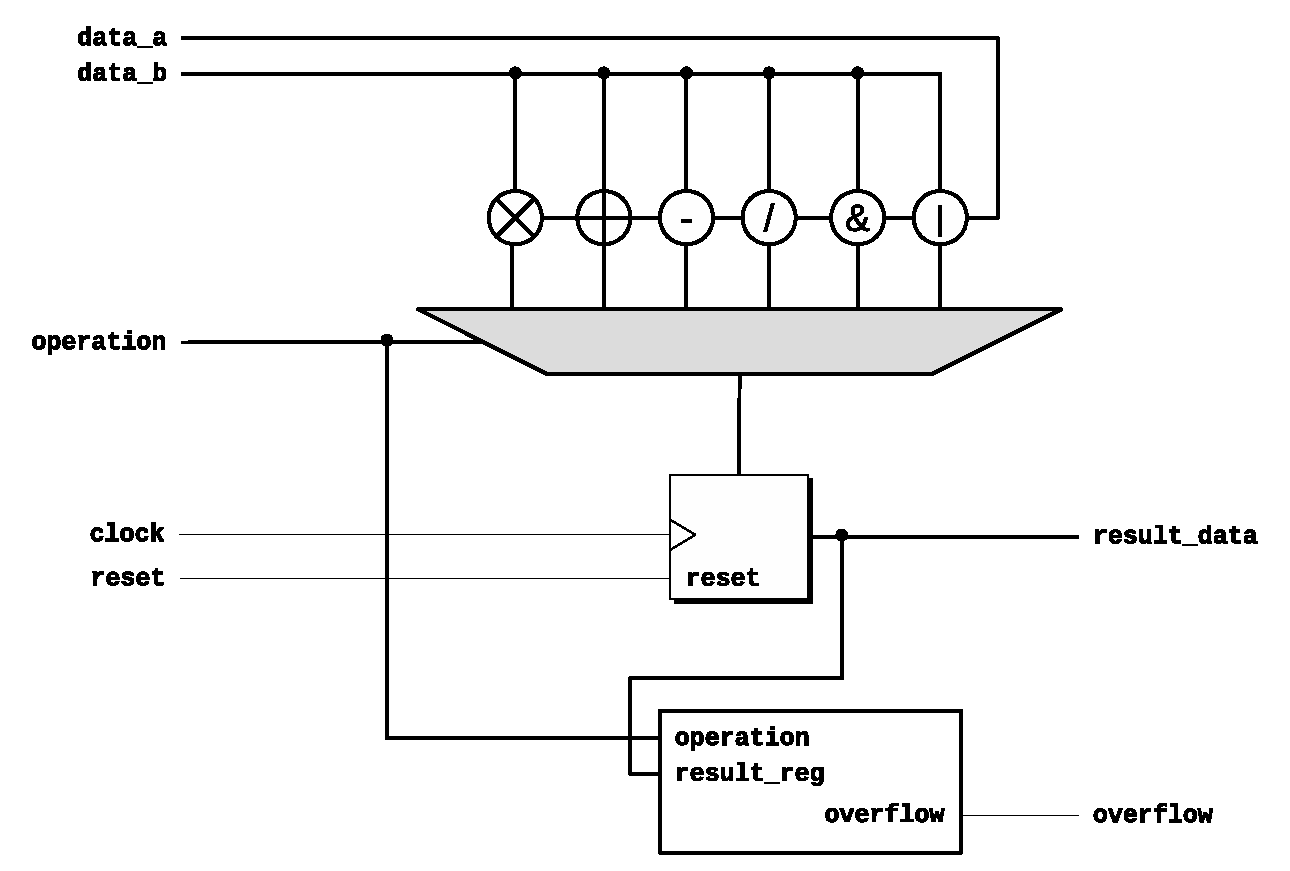
\includegraphics[width=\linewidth]{datapath/processing_datapath.eps}
      \end{figure}
    \newpage
	
	\section{Acesso à memória e write back}
	\subsection{Diagrama de Classe}
  \begin{figure}[H]
    \begin{center}
	\begin{tikzpicture}
	\umlclass[x=0,y=0]{MemoryExecute}{
	+ zero : input bit \\ 
	+ address : input bit \\ 
	+ writeData : input bit[13] \\ 
	+ memRead : input bit \\ 
	+ memWrite : input bit\\ 
	- writeBack : output bit[14]\\ 
	- writeToRegister : output bit[14]}
	{}
	\end{tikzpicture}
\end{center}
  \end{figure}

\subsection{Definições de entrada e saída}

	\begin{center}
        \begin{longtable}[pos]{| l | c | c | m{7cm} |} \hline
          \multicolumn{1}{|c|}{\cellcolor[gray]{0.9}\textbf{Nome}} & 
          \multicolumn{1}{c|}{\cellcolor[gray]{0.9}\textbf{Tamanho}} & 
          \multicolumn{1}{c|}{\cellcolor[gray]{0.9}\textbf{Direção}} &
          \multicolumn{1}{c|}{\cellcolor[gray]{0.9}\textbf{Descrição}} \\ \hline
          \endhead
          \hline
          \endlastfoot

          zero          	       & 1   & entrada   & Executa branch quando é zero.    \\ \hline
          address                  & 13  & entrada   & Endereço no qual o dado deve ser escrito.    \\ \hline
          memRead                  & 1   & entrada   & Sinal proveniente da UC que habilita leitura.    \\ \hline
          memWrite                 & 1   & entrada   & Sinal proveniente da UC que habilita escrita.    \\ \hline
          writeData      		   & 1   & entrada   & Dado a ser escrito na memória. \\ \hline
          writeBack	               & 14  & saída     & Dado proveniente da ALU que será escrito no bloco de registradores\\ \hline
          writeToRegister          & 14  & saída     & Dado do segundo operando.    \\
        \end{longtable}
      \end{center}
      
\subsection{Datapath Interno}
	
	\begin{figure}[ht]
		\begin{center}
		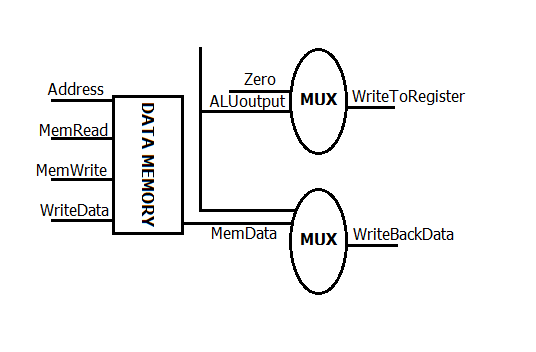
\includegraphics{./datapath/Step4_e_Step5.png}
		\caption*{Datapath dos estágios 4 e 5.}
		\end{center}
	\end{figure}

	  \section{Interface de Comunicação}

    \subsection{Diagrama de Classe}
      \begin{figure}[H]
        \centering
        \flushleft
  \begin{tikzpicture} 
    \begin{umlsystem}[x=0, fill=red!10]{Interface de Comunicação} 
      \umlactor[x=-5, y=-3]{Controle IF} 
      \umlactor[x=4, y=-5]{Controle}

      \umlusecase[name=lefunc]{Lê operação}
      \umlusecase[y=-2, name=leoperandos]{Lê operandos} 
      % \umlusecase[y=-4, name=saida,width=1.5cm]{Controla saída}
      \umlusecase[y=-4, name=operacao,width=1.5cm]{Envia operação} 
      \umlusecase[y=-6, name=operandos,width=1.5cm]{Envia operandos}

      \umlassoc{Controle IF}{lefunc}
      \umlassoc{Controle IF}{leoperandos}
      % \umlassoc{Controle IF}{saida}
      \umlassoc{Controle IF}{operacao}
      \umlassoc{Controle IF}{operandos}
      \umlassoc{operacao}{Controle}
      \umlassoc{operandos}{Controle}

    \end{umlsystem} 
  \end{tikzpicture}
      \end{figure}

    \subsection{Definições de Entrada e Saída}
      \FloatBarrier
      \begin{center}
        \begin{longtable}[pos]{| l | c | c | m{7cm} |} \hline         
          \multicolumn{1}{|c|}{\cellcolor[gray]{0.9}\textbf{Nome}} & 
          \multicolumn{1}{c|}{\cellcolor[gray]{0.9}\textbf{Tamanho}} & 
          \multicolumn{1}{c|}{\cellcolor[gray]{0.9}\textbf{Direção}} &
          \multicolumn{1}{c|}{\cellcolor[gray]{0.9}\textbf{Descrição}} \\ \hline
          \endfirsthead
          \hline
          \multicolumn{4}{|l|}%
          {{\bfseries continuação da página anterior}} \\
          \hline
          \multicolumn{1}{|c|}{\cellcolor[gray]{0.9}\textbf{Nome}} & 
          \multicolumn{1}{c|}{\cellcolor[gray]{0.9}\textbf{Tamanho}} & 
          \multicolumn{1}{c|}{\cellcolor[gray]{0.9}\textbf{Direção}} &
          \multicolumn{1}{c|}{\cellcolor[gray]{0.9}\textbf{Descrição}} \\ \hline
          \endhead

          \multicolumn{4}{|r|}{{continua na próxima página}} \\ \hline
          \endfoot

          \hline
          \endlastfoot

          clock\_in                & 1   & entrada   & Clock principal do sistema.    \\ \hline
          reset\_in                & 1   & entrada   & Sinal de reset geral do sistema.    \\ \hline
          rx\_data\_ready\_in      & 1   & entrada   & Indica que o dado foi recebido pelo controle RS232.    \\ \hline
          rx\_data\_in             & 8   & entrada   & Dado proveniente da transmissão.    \\ \hline
          data\_a\_out             & 8   & saída   & Dado do primeiro operando.    \\ \hline
          data\_b\_out             & 8   & saída   & Dado do segundo operando.    \\ \hline
          operation\_out          & TBD   & saída   & Código da operação.    \\ 
        \end{longtable}
      \end{center}    

    %\subsection{Datapath Interno}

    \subsection{Máquina de Estados}
      \begin{figure}[H]
        \centering
        \begin{tikzpicture} 
        \umlstateinitial[name=idle]
        \umlstatefinal[x=8, y=-3.2, name=final]
        \umlbasicstate[x=0, y=-4, do=counter++, name=read]{read\_data}  
        \umlbasicstate[x=4, y=-3.5, name=send]{send\_data}    

        \umltrans[arg={rx\_data\_ready\_in}]{idle}{read}
        \umltrans{read}{send}
        \umltrans{send}{final}
        \umltrans[recursive=-160|-120|3cm, recursive direction=right to bottom, arg={counter != 3}, pos=1.5]{read}{read} 
        \end{tikzpicture}    
      \end{figure}

    \begin{landscape}
      \subsection{Diagrama de Temporização}
        \begin{figure}[H]
          \centering
          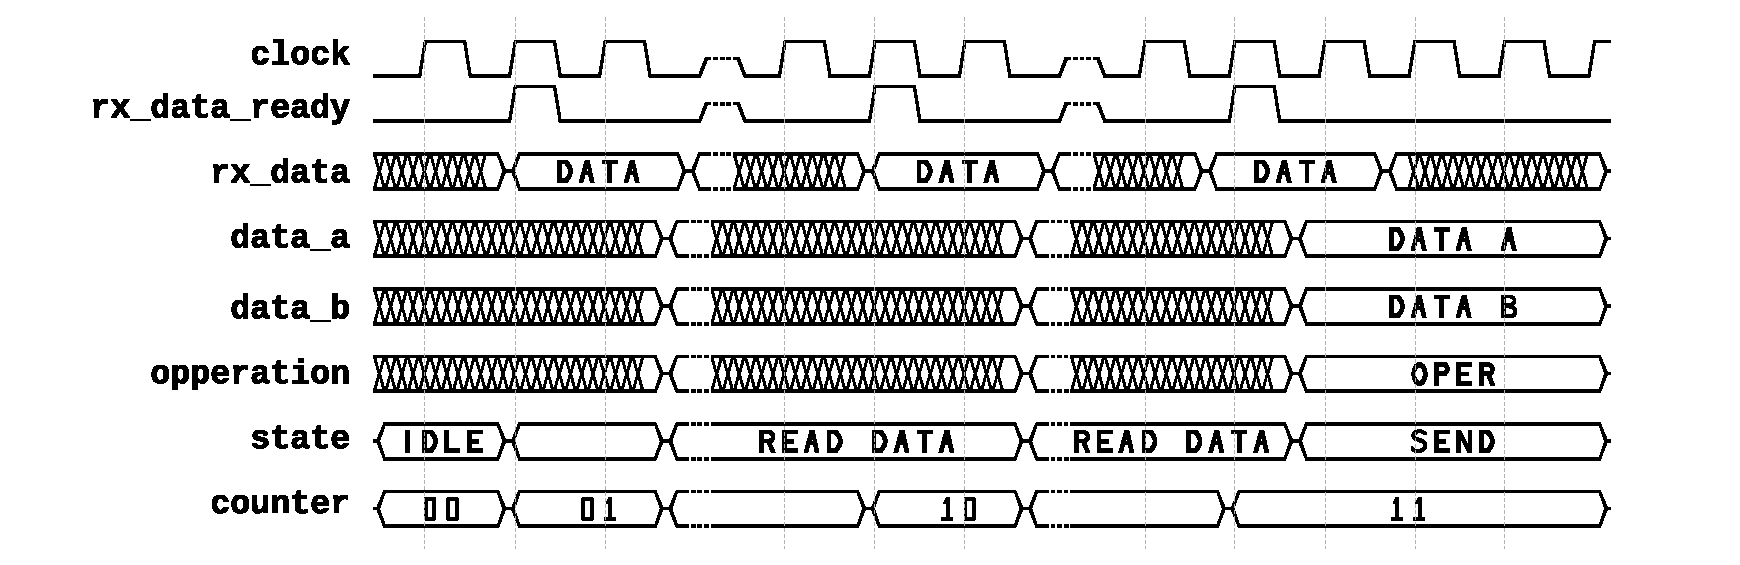
\includegraphics[width=\linewidth]{timing/comunication_timing.eps}
        \end{figure}
    \end{landscape}

% Optional bibliography section
% To use bibliograpy, first provide the ipprocess.bib file on the root folder.
% \bibliographystyle{ieeetr}
% \bibliography{ipprocess}

\end{document}
